% Options for packages loaded elsewhere
\PassOptionsToPackage{unicode}{hyperref}
\PassOptionsToPackage{hyphens}{url}
%
\documentclass[
  man]{apa6}
\usepackage{amsmath,amssymb}
\usepackage{lmodern}
\usepackage{iftex}
\ifPDFTeX
  \usepackage[T1]{fontenc}
  \usepackage[utf8]{inputenc}
  \usepackage{textcomp} % provide euro and other symbols
\else % if luatex or xetex
  \usepackage{unicode-math}
  \defaultfontfeatures{Scale=MatchLowercase}
  \defaultfontfeatures[\rmfamily]{Ligatures=TeX,Scale=1}
\fi
% Use upquote if available, for straight quotes in verbatim environments
\IfFileExists{upquote.sty}{\usepackage{upquote}}{}
\IfFileExists{microtype.sty}{% use microtype if available
  \usepackage[]{microtype}
  \UseMicrotypeSet[protrusion]{basicmath} % disable protrusion for tt fonts
}{}
\makeatletter
\@ifundefined{KOMAClassName}{% if non-KOMA class
  \IfFileExists{parskip.sty}{%
    \usepackage{parskip}
  }{% else
    \setlength{\parindent}{0pt}
    \setlength{\parskip}{6pt plus 2pt minus 1pt}}
}{% if KOMA class
  \KOMAoptions{parskip=half}}
\makeatother
\usepackage{xcolor}
\IfFileExists{xurl.sty}{\usepackage{xurl}}{} % add URL line breaks if available
\IfFileExists{bookmark.sty}{\usepackage{bookmark}}{\usepackage{hyperref}}
\hypersetup{
  pdftitle={Getting a Step Ahead: Using the Regularized Horseshoe Prior to Select Cross-Loadings in Bayesian CFA},
  pdflang={en-EN},
  hidelinks,
  pdfcreator={LaTeX via pandoc}}
\urlstyle{same} % disable monospaced font for URLs
\usepackage{graphicx}
\makeatletter
\def\maxwidth{\ifdim\Gin@nat@width>\linewidth\linewidth\else\Gin@nat@width\fi}
\def\maxheight{\ifdim\Gin@nat@height>\textheight\textheight\else\Gin@nat@height\fi}
\makeatother
% Scale images if necessary, so that they will not overflow the page
% margins by default, and it is still possible to overwrite the defaults
% using explicit options in \includegraphics[width, height, ...]{}
\setkeys{Gin}{width=\maxwidth,height=\maxheight,keepaspectratio}
% Set default figure placement to htbp
\makeatletter
\def\fps@figure{htbp}
\makeatother
\setlength{\emergencystretch}{3em} % prevent overfull lines
\providecommand{\tightlist}{%
  \setlength{\itemsep}{0pt}\setlength{\parskip}{0pt}}
\setcounter{secnumdepth}{-\maxdimen} % remove section numbering
% Make \paragraph and \subparagraph free-standing
\ifx\paragraph\undefined\else
  \let\oldparagraph\paragraph
  \renewcommand{\paragraph}[1]{\oldparagraph{#1}\mbox{}}
\fi
\ifx\subparagraph\undefined\else
  \let\oldsubparagraph\subparagraph
  \renewcommand{\subparagraph}[1]{\oldsubparagraph{#1}\mbox{}}
\fi
\newlength{\cslhangindent}
\setlength{\cslhangindent}{1.5em}
\newlength{\csllabelwidth}
\setlength{\csllabelwidth}{3em}
\newlength{\cslentryspacingunit} % times entry-spacing
\setlength{\cslentryspacingunit}{\parskip}
\newenvironment{CSLReferences}[2] % #1 hanging-ident, #2 entry spacing
 {% don't indent paragraphs
  \setlength{\parindent}{0pt}
  % turn on hanging indent if param 1 is 1
  \ifodd #1
  \let\oldpar\par
  \def\par{\hangindent=\cslhangindent\oldpar}
  \fi
  % set entry spacing
  \setlength{\parskip}{#2\cslentryspacingunit}
 }%
 {}
\usepackage{calc}
\newcommand{\CSLBlock}[1]{#1\hfill\break}
\newcommand{\CSLLeftMargin}[1]{\parbox[t]{\csllabelwidth}{#1}}
\newcommand{\CSLRightInline}[1]{\parbox[t]{\linewidth - \csllabelwidth}{#1}\break}
\newcommand{\CSLIndent}[1]{\hspace{\cslhangindent}#1}
\ifLuaTeX
\usepackage[bidi=basic]{babel}
\else
\usepackage[bidi=default]{babel}
\fi
\babelprovide[main,import]{english}
% get rid of language-specific shorthands (see #6817):
\let\LanguageShortHands\languageshorthands
\def\languageshorthands#1{}
% This preamble allows to remove the redundant title page from papaja's output.pdf
\usepackage{atbegshi}% http://ctan.org/pkg/atbegshi
\AtBeginDocument{\AtBeginShipoutNext{\AtBeginShipoutDiscard}}
% Manuscript styling
\usepackage{upgreek}
\captionsetup{font=singlespacing,justification=justified}

% Table formatting
\usepackage{longtable}
\usepackage{lscape}
% \usepackage[counterclockwise]{rotating}   % Landscape page setup for large tables
\usepackage{multirow}		% Table styling
\usepackage{tabularx}		% Control Column width
\usepackage[flushleft]{threeparttable}	% Allows for three part tables with a specified notes section
\usepackage{threeparttablex}            % Lets threeparttable work with longtable

% Create new environments so endfloat can handle them
% \newenvironment{ltable}
%   {\begin{landscape}\centering\begin{threeparttable}}
%   {\end{threeparttable}\end{landscape}}
\newenvironment{lltable}{\begin{landscape}\centering\begin{ThreePartTable}}{\end{ThreePartTable}\end{landscape}}

% Enables adjusting longtable caption width to table width
% Solution found at http://golatex.de/longtable-mit-caption-so-breit-wie-die-tabelle-t15767.html
\makeatletter
\newcommand\LastLTentrywidth{1em}
\newlength\longtablewidth
\setlength{\longtablewidth}{1in}
\newcommand{\getlongtablewidth}{\begingroup \ifcsname LT@\roman{LT@tables}\endcsname \global\longtablewidth=0pt \renewcommand{\LT@entry}[2]{\global\advance\longtablewidth by ##2\relax\gdef\LastLTentrywidth{##2}}\@nameuse{LT@\roman{LT@tables}} \fi \endgroup}

% \setlength{\parindent}{0.5in}
% \setlength{\parskip}{0pt plus 0pt minus 0pt}

% \usepackage{etoolbox}
\makeatletter
\patchcmd{\HyOrg@maketitle}
  {\section{\normalfont\normalsize\abstractname}}
  {\section*{\normalfont\normalsize\abstractname}}
  {}{\typeout{Failed to patch abstract.}}
\patchcmd{\HyOrg@maketitle}
  {\section{\protect\normalfont{\@title}}}
  {\section*{\protect\normalfont{\@title}}}
  {}{\typeout{Failed to patch title.}}
\makeatother
\shorttitle{Getting a Step Ahead: Using the Regularized Horseshoe Prior to Select Cross-Loadings in Bayesian CFA}
\keywords{\newline\indent Word count: X}
\DeclareDelayedFloatFlavor{ThreePartTable}{table}
\DeclareDelayedFloatFlavor{lltable}{table}
\DeclareDelayedFloatFlavor*{longtable}{table}
\makeatletter
\renewcommand{\efloat@iwrite}[1]{\immediate\expandafter\protected@write\csname efloat@post#1\endcsname{}}
\makeatother
\usepackage{csquotes}
\ifLuaTeX
  \usepackage{selnolig}  % disable illegal ligatures
\fi

\title{Getting a Step Ahead: Using the Regularized Horseshoe Prior to Select Cross-Loadings in Bayesian CFA}
\author{\phantom{0}}
\date{}


\affiliation{\phantom{0}}

\begin{document}
\maketitle

% move text to bottom of page
\vfill
Research Proposal \\
Michael Koch (6412157)\\
Methodology and Statistics for the Behavioral, Biomedical, and Social Sciences \\
Supervisor: Dr. Sara van Erp \\ 
Email: j.m.b.koch@students.uu.nl \\
Word Count: 695 \\
Intented Journal of Publication: Structural Equation Modeling \\
FETC permission obtained on 27'th September 2021

% make page numbers start from second page 
\pagenumbering{arabic}
\setcounter{page}{0}
\thispagestyle{empty}
% make page numbers from second page 
\pagestyle{plain}

\clearpage

\emph{Confirmatory Factor Analysis (CFA)} is an essential tool for modeling
measurement structures. Usually, all cross-loadings, factor
loadings that relate items to factors that they theoretically do not belong to, are fixed to zero to identify the model. This often leads to poor model fit,
and forces researchers to free some cross-loadings again
to improve fit, a practice that is flawed for a variety of reasons,
among which risking capitalization on chance
(MacCallum, Roznowski, \& Necowitz, 1992). As solution,
Muthen and Asparouhov (2012) proposed that rather than fixing \emph{all}
cross-loadings to zero, one should should assume that \emph{most}
cross-loadings are zero. Formally, this is achieved by setting the
so-called \emph{Small Variance Normal Prior} for the cross-loadings, which is a
normal distribution with mean zero and a very small variance (e.g.:
\(\sigma^2 = 0.01, \  \sigma^2 = 0.001\)). This prior has a large peak at zero, and very thin tails (see Figure 1). Hence, it attaches large prior mass to cross-loadings of or near zero, while attaching almost no prior mass to cross-loadings further from zero. Consequently, all cross-loadings in the model are
shrunken. The larger the prior's variance, the more
admissive the model is in the amount of deviation from zero it allows.

An issue with Muthen and Asparouhov (2012)'s approach is that not only the cross-loadings
close to zero that are considered irrelevant are shrunken to zero, as
desired, but also the ones further from zero are shrunken
towards zero, which introduces bias. The method thus requires a two-step
approach. First, the model is estimated with the Small Variance Normal Prior. Then the model
is re-estimated, with cross-loadings that have been shrunken to zero in
the previous step fixed to zero, and the remaining cross-loadings
estimated without shrinkage. This process is tedious and computationally expensive. Therefore, alternative priors need
to be identified that can outperform the Small Variance Normal Prior \emph{in a single step}.

One prior that appears as particularly promising is the \emph{Regularized Horseshoe Prior}
(Piironen \& Vehtari, 2017). This prior still has a sharp peak at zero resulting in shrinkage to zero for small coefficients (see Figure 1). However, it has much heavier tails, resulting in practically no shrinkage of larger coefficients. This prior is thus the best of both worlds, by only shrinking irrelevant parameters to zero, within one step (Piironen \& Vehtari, 2017).

\begin{figure}
\centering
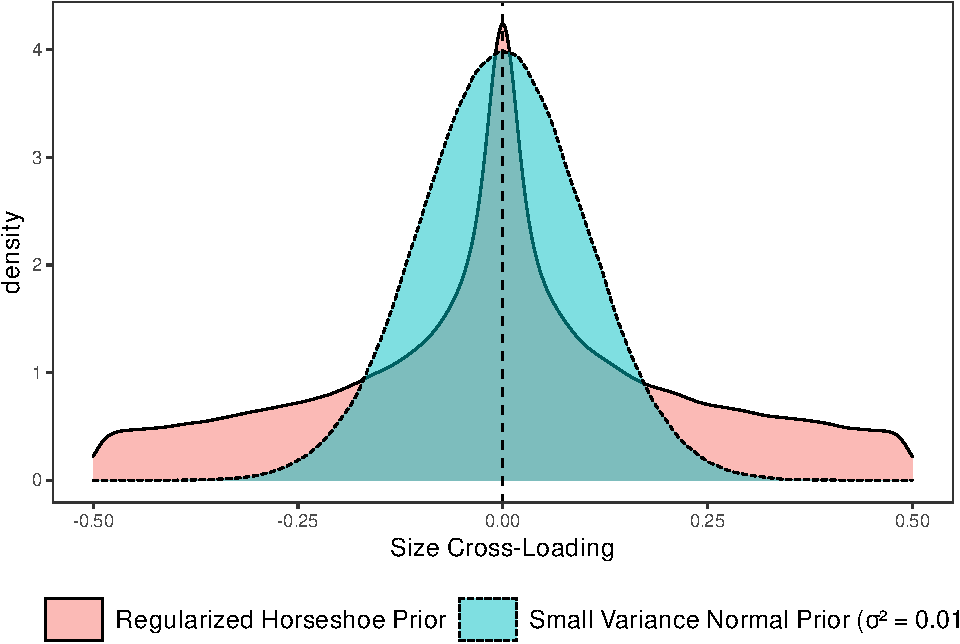
\includegraphics{JMBKoch_Proposal_files/figure-latex/unnamed-chunk-1-1.pdf}
\caption{\label{fig:unnamed-chunk-1}Density Plots of the Regularization Priors of Interest}
\end{figure}

While the Regularized Horseshoe Prior has been shown to perform well in
the selection of relevant predictors in regression
(Piironen \& Vehtari, 2017; Van Erp, Oberski, \& Mulder, 2019), no previous research
has validated its performance in selecting relevant cross-loadings in
CFA. To fill this gap, the aim of this study is to compare the
Regularized Horseshoe Prior to the Small Variance Normal Prior in their
performance in selecting the true factor structure in CFA.

\hypertarget{analytic-strategy}{%
\subsection{Analytic Strategy}\label{analytic-strategy}}

A Monte Carlo simulation study is conducted using stan
(Stan Development Team, 2021). As main outcomes, we consider the bias in the estimated cross-loadings, and the trade-off in true positives vs.~false positives in correctly identifying non-zero cross-loadings as non-zero (ROC curves). Hereby, the main criterion in selecting cross-loadings as non-zero is whether their 95\% HPD interval contains zero (Zhang, Pan, \& Ip, 2021).

We include two factor structures, one with a single, and one with three non-zero cross-loadings. Each model consists of three factors a three items. Factors are scaled by setting their means to zero and their variances to one. The correlations between all factors is set to 0.5, and the residual variance of all items to 0.3. We vary between three sample sizes (100, 200, 300), and three magnitudes of the cross-loadings (0.1, 0.2, 0.3).

Following Muthen and Asparouhov (2012) we consider three values for the hyperparameter of the Small Variance Normal Prior (\(\sigma^2\) = 0.001, 0.01, 0.1). The Regularized Horseshoe Prior has five hyperparameters, and varying all of them broadly would lead to an unfeasible number of conditions. We will therefore conduct a pilot study on a single simulated dataset to identify combinations of hyperparameters that are worth to consider in the main study.

All models will be sampled using the No-U-Turn-Sampler (Homan \& Gelman, 2014). We aim to identify a suitable chain length in the pilot study.

\clearpage

\hypertarget{references}{%
\section{References}\label{references}}

~

\begingroup
\setlength{\parindent}{-0.5in}
\setlength{\leftskip}{0.5in}

\hypertarget{refs}{}
\begin{CSLReferences}{1}{0}
\leavevmode\vadjust pre{\hypertarget{ref-homan_no-u-turn_2014}{}}%
Homan, M. D., \& Gelman, A. (2014). The {No}-{U}-turn sampler: Adaptively setting path lengths in {Hamiltonian} {Monte} {Carlo}. \emph{The Journal of Machine Learning Research}, \emph{15}(1), 1593--1623.

\leavevmode\vadjust pre{\hypertarget{ref-maccallum_model_1992}{}}%
MacCallum, R. C., Roznowski, M., \& Necowitz, L. B. (1992). Model modifications in covariance structure analysis: The problem of capitalization on chance. \emph{Psychological Bulletin}, \emph{111}(3), 490--504. \url{https://doi.org/10.1037/0033-2909.111.3.490}

\leavevmode\vadjust pre{\hypertarget{ref-muthen_bayesian_2012}{}}%
Muthen, B., \& Asparouhov, T. (2012). Bayesian {SEM}: {A} more flexible representation of substantive theory, 78. \url{https://doi.org/10.1037/a0026802}

\leavevmode\vadjust pre{\hypertarget{ref-piironen_sparsity_2017}{}}%
Piironen, J., \& Vehtari, A. (2017). Sparsity information and regularization in the horseshoe and other shrinkage priors. \emph{Electronic Journal of Statistics}, \emph{11}(2), 5018--5051. \url{https://doi.org/10.1214/17-EJS1337SI}

\leavevmode\vadjust pre{\hypertarget{ref-stan_development_team_stan_2021}{}}%
Stan Development Team. (2021). Stan {User} {Guide}. Retrieved from \url{https://mc-stan.org/docs/2_27/stan-users-guide-2_27.pdf}

\leavevmode\vadjust pre{\hypertarget{ref-van_erp_shrinkage_2019}{}}%
Van Erp, S., Oberski, D. L., \& Mulder, J. (2019). Shrinkage priors for {Bayesian} penalized regression. \emph{Journal of Mathematical Psychology}, \emph{89}, 31--50. \url{https://doi.org/10.1016/j.jmp.2018.12.004}

\leavevmode\vadjust pre{\hypertarget{ref-zhang_criteria_2021}{}}%
Zhang, L., Pan, J., \& Ip, E. H. (2021). Criteria for {Parameter} {Identification} in {Bayesian} {Lasso} {Methods} for {Covariance} {Analysis}: {Comparing} {Rules} for {Thresholding}, \emph{p} -value, and {Credible} {Interval}. \emph{Structural Equation Modeling: A Multidisciplinary Journal}, 1--10. \url{https://doi.org/10.1080/10705511.2021.1945456}

\end{CSLReferences}

\endgroup

\clearpage

\begingroup
\setlength{\parskip}{0in}
\setlength{\parindent}{-0.27in}
\setlength{\leftskip}{0.5in}

\hypertarget{additional-references}{%
\section{Additional References}\label{additional-references}}

Betancourt, Michael. 2018. ``A Conceptual Introduction to Hamiltonian Monte Carlo.'' ArXiv:1701.02434 {[}Stat{]}.

Carpenter, Bob, Andrew Gelman, Matthew D. Hoffman, Daniel Lee, Ben Goodrich, Michael Betancourt, Marcus Brubaker, Jiqiang Guo, Peter Li, and Allen Riddell. 2017. ``Stan: A Probabilistic Programming Language.'' Journal of Statistical Software 76(1):1--32. doi: 10.18637/jss.v076.i01.

Carvalho, Carlos M., Nicholas G. Polson, and James G. Scott. 2010. ``The Horseshoe Estimator for Sparse Signals.'' Biometrika 97(2):465--80. doi: 10.1093/biomet/asq017.

Ghosh, Joyee, Yingbo Li, and Robin Mitra. 2018. ``On the Use of Cauchy Prior Distributions for Bayesian Logistic Regression.'' Bayesian Analysis 13(2):359--83. doi: 10.1214/17-BA1051.

Hoerl, Arthur E., and Robert W. Kennard. 2000. ``Ridge Regression: Biased Estimation for Nonorthogonal Problems.'' Technometrics 42(1):80--86. doi: 10.2307/1271436.

Hsiang, T. C. 1975. ``A Bayesian View on Ridge Regression.'' Journal of the Royal Statistical Society. Series D (The Statistician) 24(4):267--68. doi: 10.2307/2987923.

Jacobucci, Ross, Kevin J. Grimm, and John J. McArdle. 2016. ``Regularized Structural Equation Modeling.'' Structural Equation Modeling: A Multidisciplinary Journal 23(4):555--66. doi: 10.1080/10705511.2016.1154793.

Lu, Zhao-Hua, Sy-Miin Chow, and Eric Loken. 2016. ``Bayesian Factor Analysis as a Variable-Selection Problem: Alternative Priors and Consequences.'' Multivariate Behavioral Research 51(4):519--39. doi: 10.1080/00273171.2016.1168279.

Merkle, Edgar C., Ellen Fitzsimmons, James Uanhoro, and Ben Goodrich. 2020. ``Efficient Bayesian Structural Equation Modeling in Stan.'' ArXiv:2008.07733 {[}Stat{]}.

Morris, Tim P., Ian R. White, and Michael J. Crowther. 2019. ``Using Simulation Studies to Evaluate Statistical Methods.'' Statistics in Medicine 38(11):2074--2102. doi: 10.1002/sim.8086.

Park, Trevor, and George Casella. 2008. ``The Bayesian Lasso.'' Journal of the American Statistical Association 103(482):681--86. doi: 10.1198/016214508000000337.

Tibshirani, Robert. 1996. ``Regression Shrinkage and Selection Via the Lasso.'' Journal of the Royal Statistical Society: Series B (Methodological) 58(1):267--88. doi: 10.1111/j.2517-6161.1996.tb02080.x.

Tibshirani, Robert. 2011. ``Regression Shrinkage and Selection via the Lasso: A Retrospective.'' Journal of the Royal Statistical Society. Series B (Statistical Methodology) 73(3):273--82.


\end{document}
